\documentclass{article}

\usepackage{graphicx}
\usepackage{tikz}
\usepackage{tikzsymbols}
\usetikzlibrary{calc,patterns,shapes.geometric}
\pagestyle{empty}
\usepackage[margin=0pt]{geometry}
\geometry{papersize={14in,12in}}

\def\centerarc[#1](#2)(#3:#4:#5){\draw[#1] ($(#2)+({#5*cos(#3)},{#5*sin(#3)})$) arc (#3:#4:#5);}

\begin{document}
	\begin{figure}
		\centering
		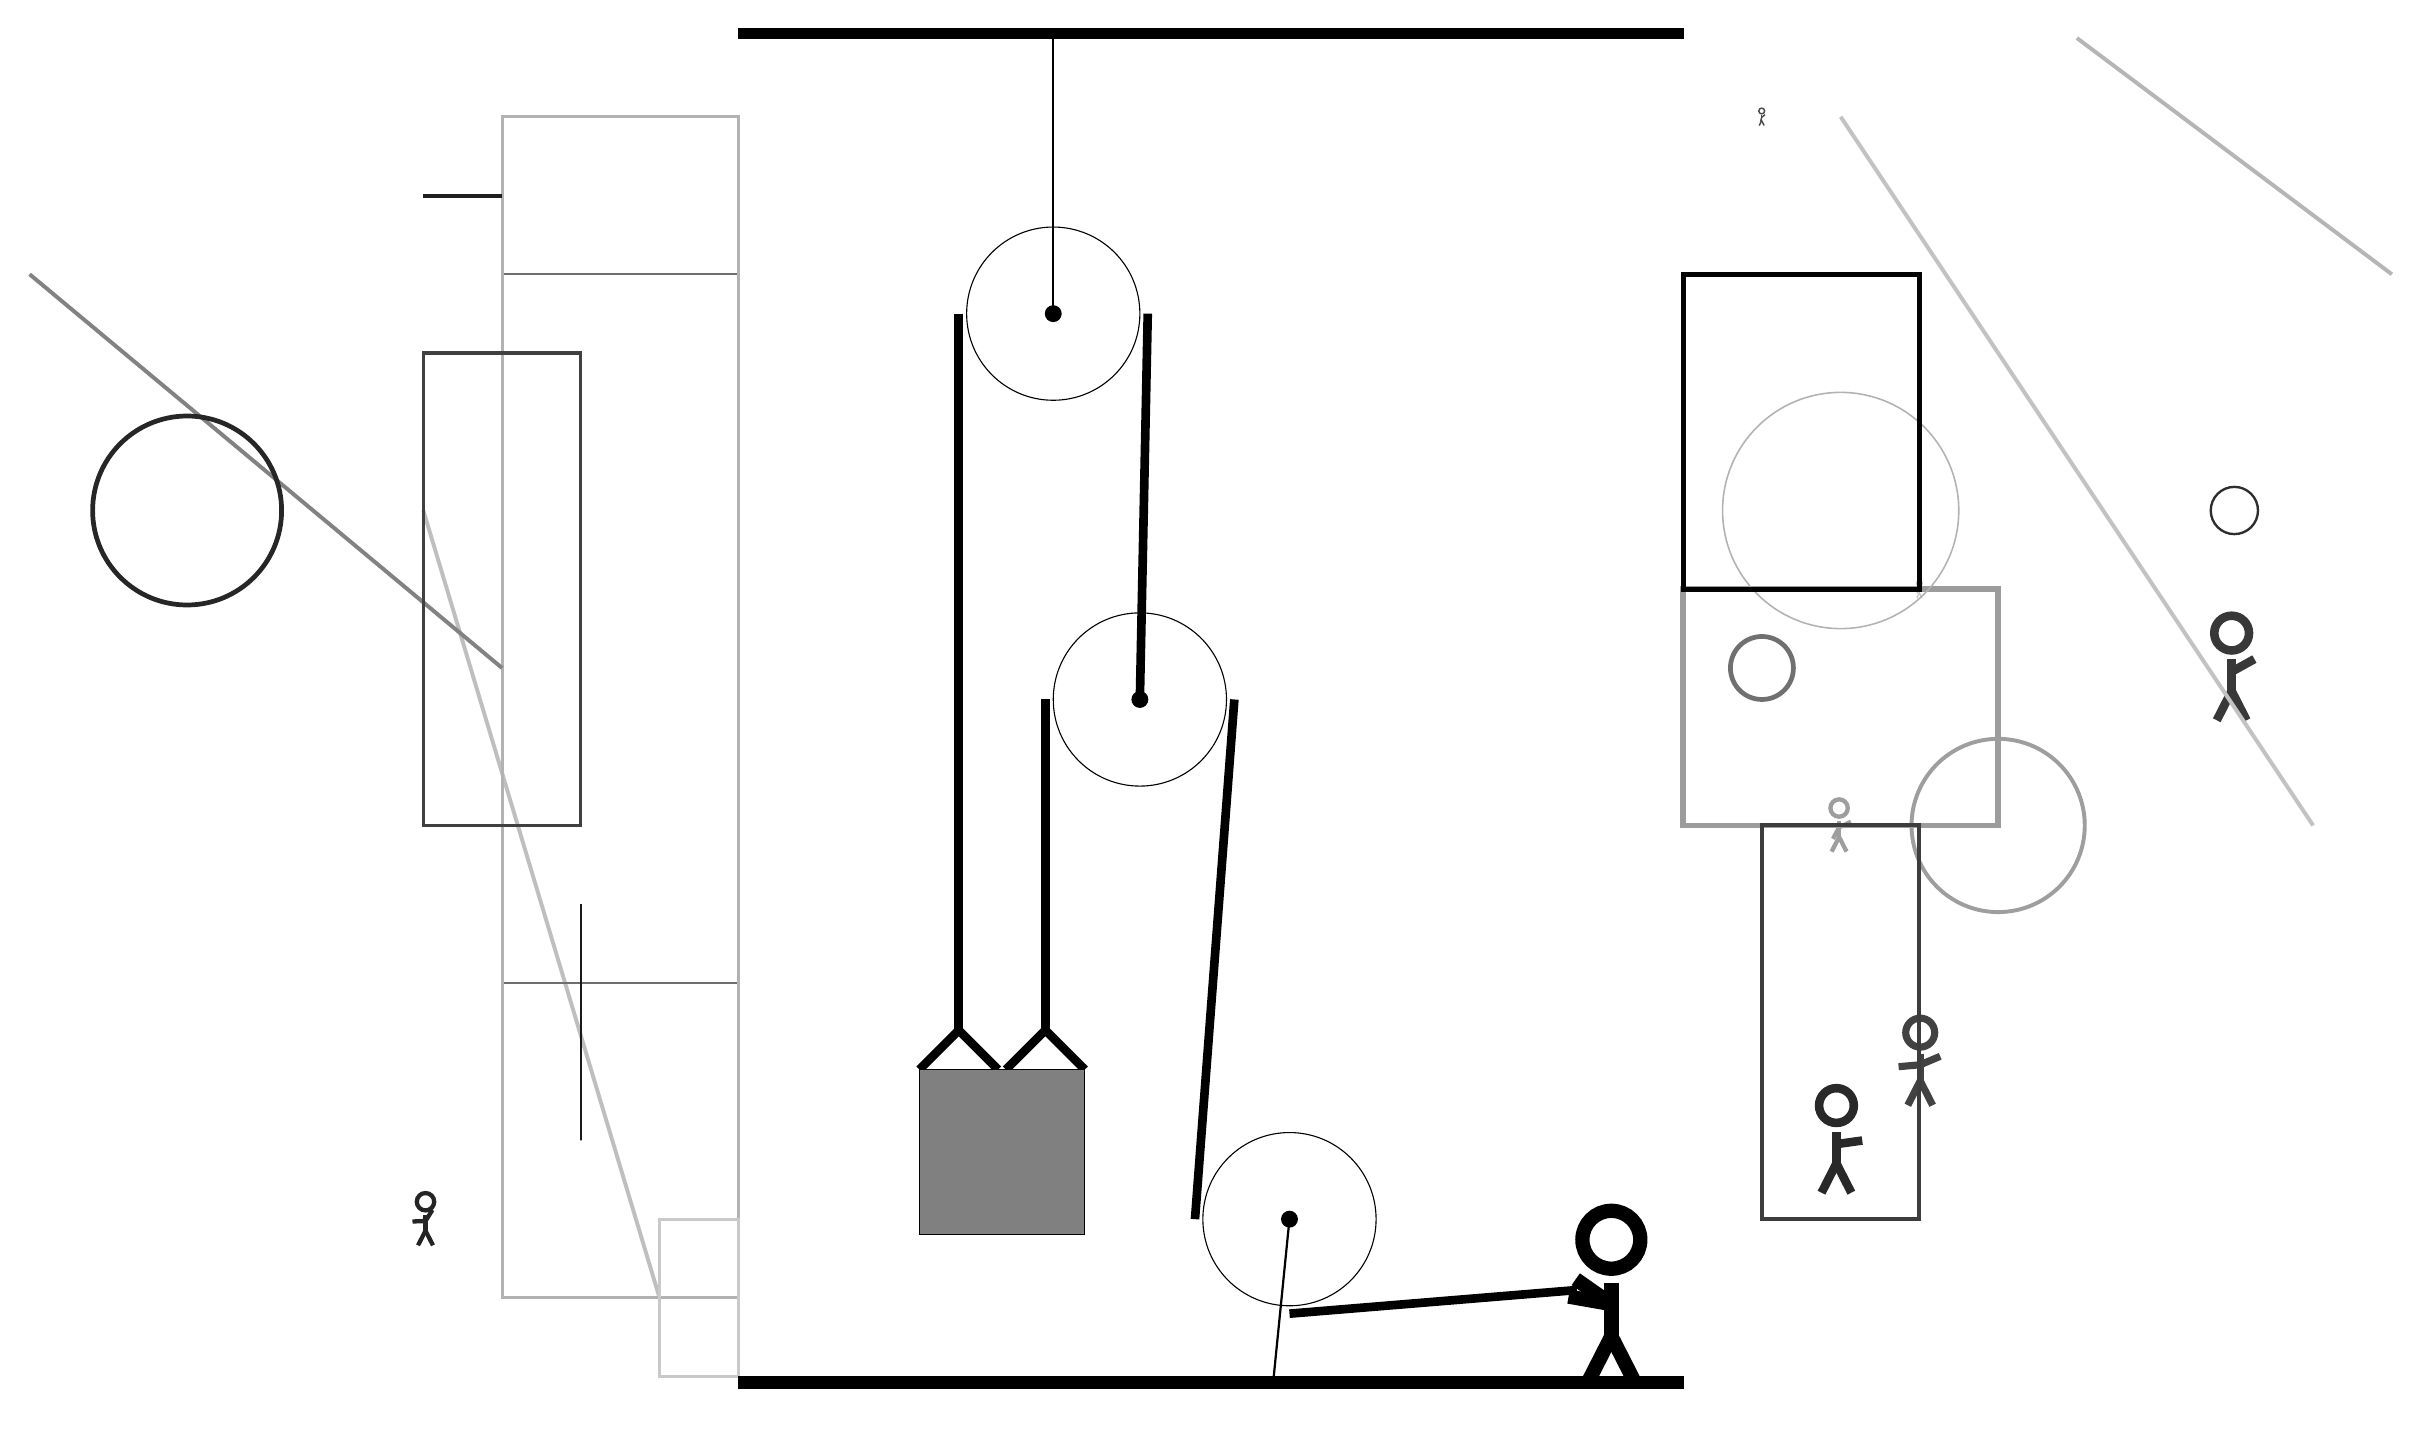
\begin{tikzpicture}
			%%%%% START %%%%%
			
			\draw[fill=black] (-2, 14) rectangle (10, 14.125);
			
			\draw[line width=0.5mm, color=black!25](-6, 8) -- (-3, -2);
			
			\node[line width=0.5mm, color=black!71] at (11, 13) {\Strichmaxerl[1][74][40]};
			\draw[line width=0.7mm, color=black!39] (10, 4) rectangle (14, 7);
			\draw[line width=0.2mm, color=black!57] (-2, 2) rectangle (-5, 11);
			\node[line width=0.3mm, color=black!78] at (17, 6) {\Strichmaxerl[6][90][29]};
			\node[line width=0.7mm, color=black!38] at (12, 4) {\Strichmaxerl[3][62][25]};
			\node[line width=0.3mm, color=black!22] at (13, 7) {\Strichmaxerl[1][56][55]};
			\draw[line width=0.5mm, color=black!29](15, 14) -- (19, 11);
			\draw[line width=0.3mm, color=black!90] (-4, 3) rectangle (-4, 0);
			
			\draw [line width=0.6mm, color=black!56](11, 6) circle (0.4);
			\node[line width=0.7mm, color=black!74] at (13, 1) {\Strichmaxerl[5][5][23]};
			\draw[line width=0.5mm, color=black!24](12, 13) -- (18, 4);
			\draw [line width=0.2mm, color=black!30](12, 8) circle (1.5);
			\draw[line width=0.6mm, color=black!99] (10, 11) rectangle (13, 7);
			\draw[line width=0.4mm, color=black!30] (-2, 13) rectangle (-5, -2);
			\draw[line width=0.5mm, color=black!88](-6, 12) -- (-5, 12);
			
			\draw[line width=0.5mm, color=black!49](-5, 6) -- (-11, 11);
			
			\draw [line width=0.5mm, color=black!38](14, 4) circle (1.1);
			\draw [line width=0.6mm, color=black!85](-9, 8) circle (1.2);
			\draw[line width=0.5mm, color=black!76] (11, 4) rectangle (13, -1);
			\node[line width=0.3mm, color=black!84] at (12, 0) {\Strichmaxerl[6][90][8]};
			
			\draw [line width=0.3mm, color=black!82](17, 8) circle (0.3);
			
			\node[line width=0.3mm, color=black!86] at (-6, -1) {\Strichmaxerl[3][2][58]};
			\draw[line width=0.4mm, color=black!75] (-4, 4) rectangle (-6, 10);
			\draw[line width=0.4mm, color=black!21] (-3, -1) rectangle (-2, -3);
			
			\draw (2, 10.5) circle (1.1);
			\draw[fill=black] (2, 10.5) circle (0.1);
			\draw[thick] (2, 10.5) -- (2, 14);
			
			\draw (3.1, 5.6) circle (1.1);
			\draw[fill=black] (3.1, 5.6) circle (0.1);
			
			\draw (5, -1) circle (1.1);
			\draw[fill=black] (5, -1) circle (0.1);
			\draw[thick] (5, -1) -- (4.8, -3);
			
			\draw[line width = 1.1mm]  (0.3, 0.9) -- (0.8, 1.4) -- (1.3, 0.9);
			\draw[line width = 1.1mm]  (1.4, 0.9) -- (1.9, 1.4) -- (2.4, 0.9);
			\draw[fill=black!50] (0.3, 0.9) rectangle (2.4, -1.2);
			
			\draw[line width = 1.1mm] (0.8, 10.5) -- (0.8, 1.4);
			\centerarc[line width = 1.1mm](2, 10.5)(0:180:1.2000000000000002);
			\draw[line width = 1.1mm] (3.2, 10.5) -- (3.1, 5.6);
			\draw[line width = 1.1mm] (1.9, 5.6) -- (1.9, 1.4);
			\centerarc[line width = 1.1mm](3.1, 5.6)(0:180:1.2000000000000002);
			\draw[line width = 1.1mm] (4.3, 5.6) -- (3.8, -1);
			\centerarc[line width = 1.1mm](5, -1)(180:270:1.2000000000000002);
			\draw[line width = 1.1mm] (5, -2.2) -- (8.65, -1.9);
			
			\node at (9, -2) {\Strichmaxerl[10][-35][170]};
			
			\draw[fill=black] (-2, -3) rectangle (10, -3.15);
			
			%%%%% END %%%%%
		\end{tikzpicture}
	\end{figure}	
\end{document}